\documentclass[conference,letterpaper]{IEEEtran}
\IEEEoverridecommandlockouts
\usepackage{cite}
\usepackage{amsmath,amssymb,amsfonts}
\usepackage{graphicx}
\usepackage{url}
\usepackage{xcolor}
\usepackage{booktabs,tabularx,array}
\usepackage{balance}
\usepackage{placeins}
\usepackage{float}
\usepackage{needspace}
\usepackage[hidelinks]{hyperref}

% Conference-specific checklist overrides the IEEEtran caption/citation defaults.
\renewcommand{\figurename}{Figure}
\renewcommand{\tablename}{Table}
\renewcommand{\thetable}{\arabic{table}}
\let\citeplain\cite
\renewcommand{\cite}[1]{\textsuperscript{\citeplain{#1}}}

\graphicspath{{figures/}}
\interdisplaylinepenalty=2500

\title{A Shared LSTM Forecast for 3-D UAV Planning with Coupled MPC--DWA in Dynamic Obstacle Fields}
\author{\IEEEauthorblockN{Zhenhui Fu\textsuperscript{*}}
\IEEEauthorblockA{Beijing University of Chemical Technology\\
Beijing 100029, China\\
\textsuperscript{*}Corresponding author: 2025090094@buct.edu.cn}}

\begin{document}
\maketitle

\begin{abstract}
First, a UAV must avoid moving obstacles in three dimensions even when turns, acceleration and pauses make their motion difficult to predict. Second, the method couples model predictive control (MPC) and the dynamic window approach (DWA) through one causal long short-term memory (LSTM) forecast. MPC uses it to optimize a route; DWA screens reachable actions and bounds MPC's first command. Then, in a frozen 500-scene comparison with a 1-s DWA screen, shared LSTM achieved collision-free goal arrival in 936/1,500 runs (62.4\%), versus 836/1,500 (55.7\%) when only DWA received LSTM. The paired difference was 6.7 percentage points (95\% scene-cluster confidence interval, 4.2--9.2). In a separate 100-scene exploratory evaluation with a 3-s DWA screen, sharing reached 73.7\%; its contrast with DWA-only LSTM was inconclusive. Standalone MPC-CV reached 92.0\%, the highest rate in that evaluation. Finally, the simulations support a protocol-specific benefit of forecast sharing, not general controller superiority or real-flight performance.
\end{abstract}

\begin{IEEEkeywords}
UAV, 3D path planning, dynamic obstacles, LSTM, model predictive control, dynamic window approach
\end{IEEEkeywords}

\section{Introduction}
Unmanned aerial vehicles (UAVs) must avoid obstacles that move during flight. Turns, acceleration and pauses make recent positions unreliable guides to what happens next. Model predictive control (MPC) optimizes a short future route, whereas the dynamic window approach (DWA) selects a feasible next action \cite{mayne2000,fox1997}. Predictive UAV planners already use obstacle-motion forecasts in route optimization \cite{olcay2024,xu2025}; here we test where one causal long short-term memory (LSTM) forecast should enter a coupled MPC--DWA loop. The main comparison tests whether also giving MPC the forecast already used by DWA changes outcomes; CV-only, MPC-only-LSTM, DWA-only-LSTM and standalone arms provide context.

\section{Problem Formulation}
We model the UAV as a collision sphere in a bounded three-dimensional workspace with a start, goal and moving spherical obstacles. Each obstacle has an observed center, radius and time-varying path; future ground-truth positions are hidden from the planner. At each update, it chooses a dynamically feasible action to reach the goal without intersecting an obstacle along the simulated motion. Figure~\ref{fig:scenario} shows the scene geometry; recorded planner paths are compared separately.

\begin{figure}[!hb]
\centering
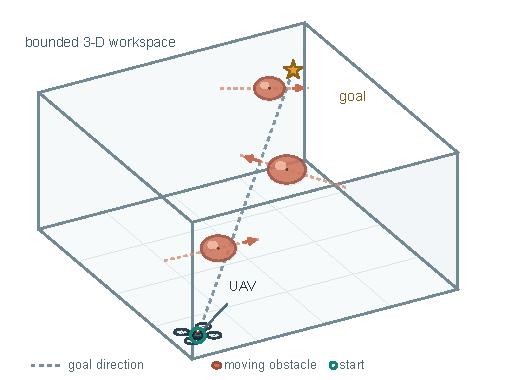
\includegraphics[width=0.90\columnwidth]{scenario_schematic.pdf}
\caption{Problem geometry: the quadrotor is centered at the start and moves toward the goal among spherical obstacles following prescribed paths (arrows). The dashed line marks the direct start-to-goal direction, not a simulated route; planner trajectories appear separately in Figure~\ref{fig:routes}.}
\label{fig:scenario}
\end{figure}

\FloatBarrier
\section{Planning Method}
With the scene defined, the planner uses one causal obstacle forecast to align route optimization with near-term action screening.

\subsection{Core equations}
The following compact relations define the state update, obstacle forecast and quantities used by the planners.
The UAV is represented by its position, speed, pitch and yaw. The signed distance between its collision sphere and obstacle $j$ is
\begingroup\small
\begin{equation}
\begin{aligned}
\mathbf h_t&=[\cos\theta_t\cos\psi_t,\cos\theta_t\sin\psi_t,\sin\theta_t]^{\mathsf T},\\
\mathbf p_{t+1}&=\mathbf p_t+\Delta t\,v_t\mathbf h_t,\\
v_{t+1}&=v_t+\frac{\Delta t}{\tau_v}(v_{c,t}-v_t),\\
\theta_{t+1}&=\theta_t+\Delta t\,\omega_{\theta,t},\quad
\psi_{t+1}=\psi_t+\Delta t\,\omega_{\psi,t},\\
\hat d_{j,k}&=\|\mathbf p_{t+k|t}-\hat{\mathbf o}_{j,t+k|t}\|_2-r_u-r_j.
\end{aligned}
\label{eq:model}
\end{equation}
\endgroup
Here $t$ is the current step, $k$ a future step, and $j=1,\ldots,M$ indexes the $M$ obstacles. The unit direction $\mathbf h_t$ follows the UAV's pitch $\theta_t$ and yaw $\psi_t$. The update period is $\Delta t=0.1$ s; $\tau_v$ is the speed-response time; $v_c,\omega_\theta,\omega_\psi$ are commanded speed, pitch rate and yaw rate. In the clearance term, $\mathbf p_{t+k|t}$ and $\hat{\mathbf o}_{j,t+k|t}$ are the predicted UAV position and obstacle centre at step $k$. The UAV and obstacle radii are $r_u$ and $r_j$. Positive $\hat d_{j,k}$ means separation, zero contact, and negative overlap.

At each update, the causal LSTM \cite{hochreiter1997} maps ten obstacle observations to thirty 3-D offsets from the latest observed centre:
\begingroup\small
\begin{equation}
\begin{aligned}
\mathbf q_{j,s}&=[\mathbf o_{j,s}^{\mathsf T},\mathbf v_{j,s}^{\mathsf T},\cos\chi_{j,s},\sin\chi_{j,s}]^{\mathsf T},\\
\hat{\mathbf o}^{\rm LSTM}_{j,t+k|t}&=\mathbf o^{\rm obs}_{j,t}+[f_{\Theta}(\mathbf q_{j,t-9:t})]_k.
\end{aligned}
\label{eq:forecast}
\end{equation}
\endgroup
Here $s$ indexes history and $k=1,\ldots,30$ indexes the forecast steps. The position $\mathbf o$ and velocity $\mathbf v$ in $\mathbf q$ are observed obstacle inputs, followed by sine and cosine of heading $\chi$; thus $\mathbf q$ has eight features. The trained network $f_\Theta$ uses learned weights $\Theta$ and outputs a 3-D offset for each future step; $[\cdot]_k$ denotes offset $k$. Ten observations span 0.9 s and the 30 outputs span 3 s. The forecast is causal and each offset is anchored to the latest observed centre, not cumulatively summed. At startup, the earliest state fills missing history. CV baselines extrapolate from the latest two observed positions (zero initial velocity when only one is available); position hold repeats the latest centre. Training details are in Supplementary Methods.

MPC uses the forecast over its 30-step horizon to minimize goal error, control effort and changes, route deviation, and obstacle-clearance penalties:
\begingroup\small
\begin{equation}
\begin{aligned}
\min_{\mathbf u_{1:30}}J_{\rm MPC}={}&
\sum_{k=0}^{29}w_p\|\mathbf p_{t+k|t}-\mathbf g\|_2^2\\
&+w_f\|\mathbf p_{t+30|t}-\mathbf g\|_2^2+w_rJ_r\\
&+\sum_{k=1}^{30}w_u\|\mathbf u_k\|_2^2
+w_{\Delta u}\sum_{k=2}^{30}\|\mathbf u_k-\mathbf u_{k-1}\|_2^2\\
&+\sum_{k=1}^{30}\sum_j
\left(w_o[-\hat d_{j,k}]_+^2+w_s[d_{\rm soft}-\hat d_{j,k}]_+^2\right),\\
\text{s.t. }&\mathbf x_{t+k|t}=f(\mathbf x_{t+k-1|t},\mathbf u_k),\quad
\mathbf u_1\in\mathcal U_t\ \text{if }\mathcal A_t\ne\varnothing.
\end{aligned}
\label{eq:mpc}
\end{equation}
\endgroup
Here $\mathbf u_{1:30}$ denotes the sequence of 30 future commands; $\mathbf x=[\mathbf p^{\mathsf T},\theta,\psi,v]^{\mathsf T}$ is the position--pitch--yaw--speed state, $\mathbf u_k=[v_{c,k},\omega_{\theta,k},\omega_{\psi,k}]^{\mathsf T}$ is command $k$, $\mathbf g$ is the goal, and $f$ is the discrete state transition in Eq.~(1). $J_r$ sums squared cross-track distances from the direct start-to-goal line. The weights $w_p,w_f,w_r,w_u,w_{\Delta u},w_o,w_s$ apply to stage goal error, terminal error, route deviation, control effort, command changes, overlap and clearance below $d_{\rm soft}=0.35$ m. The positive-part function is $[x]_+=\max(0,x)$. Physical command and rate limits remain active; because the implementation squares native command units, the effort term is a heuristic cost rather than physical energy. Full geometric definitions, weights and limits are in Supplementary Methods S1.1. These clearance penalties are soft, so they do not certify safety by themselves.

Trust allocates DWA samples between guided and exploratory actions using safety, goal progress, agreement with the previous MPC guide, and control smoothness:
\begingroup\small
\begin{equation}
\begin{aligned}
\tau&=\sigma_s\tau_{\rm sa}+\sigma_g\tau_g+\sigma_t\tau_{\rm ref}+\sigma_m\tau_{\rm sm},\\
\tau_{\rm ref}&=\exp(-\alpha_T\Delta_p),\\
B&=\operatorname{round}[300(1+\alpha e^{-\beta\tau})],\\
B_g&=\operatorname{round}(B\tau),\quad B_e=B-B_g.
\end{aligned}
\label{eq:trust}
\end{equation}
\endgroup
The scores $\tau_{\rm sa},\tau_g,\tau_{\rm ref},\tau_{\rm sm}$ measure safety, goal progress, agreement with the previous MPC guide and control smoothness; their nonnegative weights $\sigma_s,\sigma_g,\sigma_t,\sigma_m$ sum to one. The mismatch $\Delta_p$ is the distance from the current UAV position to the guide's first predicted position, and $\alpha_T=3~\mathrm{m}^{-1}$. The 300-based budget $B$ splits into guided samples $B_g$ and exploratory samples $B_e$; higher trust raises the guided share while reducing the total budget. The weights were selected in a separate 4,320-episode Stage-1 development sweep (six vectors, five integrated arms, 48 scenes and three seeds). The selected vector $[0.15,0.15,0.15,0.55]$ maximized the five-arm equal-weight mean collision-free goal-arrival rate (0.8042) in that development set, not a held-out test. The historical 1-s benchmark retained inherited weights $[0.35,0.30,0.15,0.20]$, untuned on its 500 scenes. Budget settings $\alpha=1$, $\beta=3$ and reference-decay setting $\alpha_T=3~\mathrm{m}^{-1}$ are fixed implementation values; planned Stage-2 calibration was incomplete. Full score definitions and parameters are in Supplementary Methods S1.2.

DWA rejects unsafe rollouts, scores the survivors, and uses their control range to bound MPC's first input:
\begingroup\small
\begin{equation}
\begin{aligned}
\mathcal A_t&=\{b\in\mathcal B_t:d_{\min}^{(b)}>0.25~\mathrm m,\ \mathcal C_b=1,\\
&\hspace{1em}(v_{\rm end}^{(b)})^2\leq2a_{\max}d_{\min}^{(b)}\},\quad
b^*=\arg\max_{b\in\mathcal A_t}S_b,\\
u_{i,t}^{-}&=\max\!\left(u_i^{\min},\min_{b\in\mathcal A_t}u_i^{(b)}-\delta\right),\\
u_{i,t}^{+}&=\min\!\left(u_i^{\max},\max_{b\in\mathcal A_t}u_i^{(b)}+\delta\right),\\
\mathcal U_t&=\prod_{i=1}^{3}[u_{i,t}^{-},u_{i,t}^{+}],\quad \delta=0.1.
\end{aligned}
\label{eq:dwa}
\end{equation}
\endgroup
Here $\mathcal B_t$ is the sampled set, and $d_{\min}^{(b)}$ is candidate $b$'s minimum clearance over the active DWA screen and all obstacles. The frozen benchmark screens the first 10 forecast states (1 s); the separate exploratory evaluation screens all 30 (3 s). MPC uses a 30-step (3-s) horizon in both. The indicator $\mathcal C_b=1$ means the rollout remains inside the flight corridor. The terminal speed is $v_{\rm end}^{(b)}$ and available deceleration is $a_{\max}=1.0$ m s$^{-2}$. $S_b$ ranks MPC-endpoint agreement, heading, speed, obstacle clearance and vertical profile. For a nonempty safe set $\mathcal A_t$, its per-coordinate extrema, expanded by $\delta=0.1$ in each control coordinate and clipped to its physical limits $u_i^{\min},u_i^{\max}$, form $\mathcal U_t$; this numerical margin is an implementation heuristic because the controls have different units. The DWA action is executed unless optional lateral recentering is triggered; the adjusted rollout is re-screened, and failure reverts to the original screened action. The envelope constrains only MPC's first command and is not a safety certificate. If the normal safe set is empty, emergency actions are screened; if none passes, the simulator stops. Full scores and fallback logic are in Supplementary Methods S1.2--S1.4.

\subsection{How the shared forecast is used}
Every 0.1 s, the causal LSTM produces one time-aligned 3-s obstacle forecast for both planners. MPC uses all 30 positions in its route cost; DWA screens the first 10 in the frozen benchmark and all 30 in the separate exploratory evaluation. This division is deliberate: MPC plans around predicted future conflicts, while DWA checks whether the next command is reachable and passes local rollout gates. Sharing aligns both checks to the same predicted obstacle motion. Passing DWA controls constrain MPC's first command on re-solve, while the screened DWA action is executed. Because the MPC guide also sets DWA's trust-based sampling budget, changing the forecast supplied to MPC can change both the route cost and DWA's guided/exploratory allocation. The paired contrast therefore estimates the closed-loop effect of enabling MPC's LSTM input, not the isolated effect of the MPC forecast penalty. In the DWA-only arm, MPC instead uses latest-position hold in the historical benchmark and its configured CV input in the 3-s ablation. Figure~\ref{fig:algorithm} summarizes the cycle; Supplementary Methods S1.4 gives the full fallback logic.

\begin{figure}[!t]
\centering
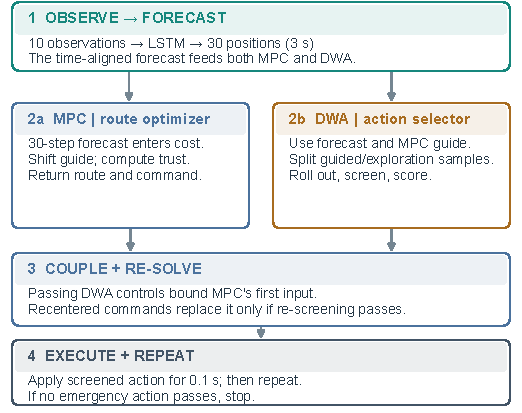
\includegraphics[width=0.92\columnwidth]{algorithm_main_pseudocode.pdf}
\caption{Numbered modules in one 0.1-s receding-horizon update. One causal LSTM forecast feeds MPC's route guide and DWA's action screen; the MPC guide also informs DWA sampling. The branches show normal safe-action selection, optional re-screened recentering, and emergency screening with stop if no candidate passes.}
\label{fig:algorithm}
\end{figure}

\section{Simulation and Results}
We report the frozen matched comparison first and the separate exploratory evaluation second; their protocols and scene banks are not pooled.

Under the frozen 1-s DWA/3-s MPC protocol with inherited weights, 500 scenes and three matched seeds compared shared LSTM with DWA-only LSTM. DWA received LSTM forecasts in both arms; only the shared arm also supplied them to MPC. Safe arrival was 936/1,500 (62.4\%) versus 836/1,500 (55.7\%), a paired gain of 6.7 percentage points (95\% scene-cluster CI, 4.2--9.2). These 3,000 runs are part of the 7,500-run benchmark, not an extra sample. In the same protocol, standalone DWA+LSTM and MPC+LSTM reached 82.4\% and 95.2\%, respectively, while the latest-position-hold reconstruction reached 2.2\% (Fig.~\ref{fig:rates}a; Supplementary Methods S4). Thus, forecast sharing improved on DWA-only input but did not outperform the independent controllers overall.

The separate exploratory evaluation comprised 2,100 episodes: seven arms, 100 distinct scenes and three matched seeds per scene. It used 0.1-s updates, 3-s MPC/DWA horizons and a 650-step limit. The arms were standalone DWA-CV and MPC-CV, coupled MPC--DWA-CV, LSTM to MPC only, LSTM to DWA only, shared LSTM and latest-position hold. Arrival required goal tolerance without swept-path contact; seeds were averaged within scene, and 20,000 scene-cluster bootstrap resamples formed simultaneous max-|t| intervals for six shared-versus-comparator contrasts. Shared LSTM reached in 221/300 runs (73.7\%), compared with 276/300 (92.0\%) for standalone MPC-CV, the highest rate; MPC-CV also had 15 swept-contact runs. Its difference from DWA-only LSTM was inconclusive; it exceeded position hold by 16.3 points (95\% CI, 5.1--27.6) but was 18.3 points below MPC-CV (95\% CI, -29.6 to -7.0). This evaluation also does not establish an overall best controller (Fig.~\ref{fig:rates}b; Supplementary Table S12).

\begin{figure}[!htbp]
\centering
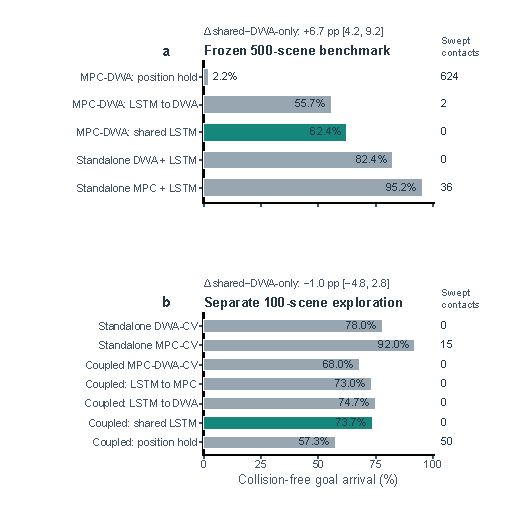
\includegraphics[width=0.98\columnwidth]{seven_method_outcomes_main.pdf}
\caption{Collision-free goal-arrival rates in two separate protocols. (a) Frozen five-controller benchmark: 500 scenes, three matched seeds, $n=1{,}500$ per method and a 1-s DWA screen. (b) Separate seven-method exploration: 100 scenes, three matched seeds, $n=300$ per method and a 3-s screen. Bars are point estimates; the paired shared-minus-DWA-only contrast is shown above each panel: +6.7 percentage points (95\% scene-cluster CI 4.2--9.2) in (a), and -1.0 points (simultaneous 95\% CI -4.8--2.8) in (b). The right column gives swept contacts for each method. The highest-rate method differs by protocol; panels are not pooled.}
\label{fig:rates}
\end{figure}

A matched route from the separate seven-method evaluation (scene 72, sampling seed 2) is shown in Fig.~\ref{fig:routes}. Shared LSTM and DWA-CV arrived safely in this example; the other five did not achieve collision-free goal arrival. This single case illustrates route geometry, not the aggregate ranking.

\begin{figure}[!t]
\centering
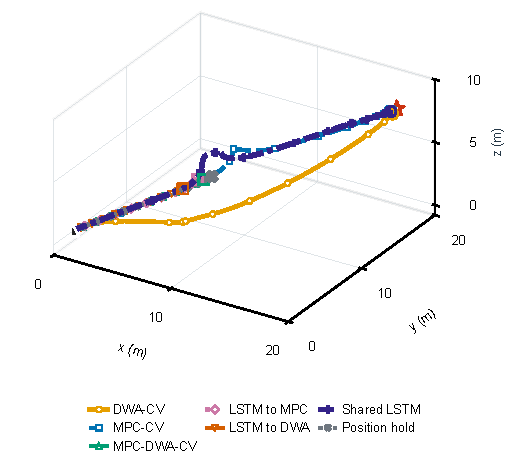
\includegraphics[width=0.98\columnwidth]{route_comparison_seven_method_scene72_seed2_singlecol.pdf}
\caption{Seven recorded paths in one matched case (scene 72, seed 2). Shared LSTM and DWA-CV arrived without swept contact; MPC-CV reached goal tolerance but had swept contact; the other methods stopped or contacted earlier. Lines join saved states without interpolation, smoothing or extension, and end at recorded terminal points. Markers show outcome, not contact location. This example is descriptive; aggregate rates appear in Fig.~\ref{fig:rates}b.}
\label{fig:routes}
\end{figure}

\section{Discussion}
The two protocols indicate a protocol-specific benefit: forecast sharing raised safe arrival in the frozen 1-s screen comparison, but not in the 3-s exploratory comparison; standalone MPC-CV had the highest rate there. Because scene banks, trust weights and horizons also differed, these studies do not isolate the source of that difference. LSTM uses simulator-recorded obstacle velocity and heading, whereas CV estimates velocity from positions, so the contrast concerns configured input pipelines as well as predictors. Prescribed tracks, point forecasts and no flight tests limit generalization.
\Needspace{7\baselineskip}
\begin{samepage}
\section{Conclusion}
In simulation, shared LSTM increased collision-free arrival by 6.7 percentage points over DWA-only input in the frozen 500-scene, 1-s DWA comparison. In the separate 3-s evaluation, standalone MPC-CV had the highest rate, and the shared-versus-DWA-only contrast was inconclusive.
\end{samepage}

\balance
\bibliographystyle{IEEEtran}
{\scriptsize\bibliography{references}}
\end{document}





